\documentclass[conference,10pt]{IEEEtran}
\IEEEoverridecommandlockouts
\usepackage{amsmath,amssymb}
\usepackage{graphicx}
\usepackage{booktabs}
\usepackage{multirow}
\usepackage{xcolor}
\usepackage{cite}
\usepackage{url}
\usepackage{bm}
\usepackage{array}
\usepackage{placeins}
\usepackage[hidelinks]{hyperref}
\graphicspath{{figures/}}
\raggedbottom
\renewcommand{\topfraction}{0.85}
\renewcommand{\dbltopfraction}{0.85}
\renewcommand{\textfraction}{0.1}
\renewcommand{\floatpagefraction}{0.75}
\renewcommand{\dblfloatpagefraction}{0.75}
\setcounter{topnumber}{3}
\setcounter{dbltopnumber}{2}
\setcounter{totalnumber}{5}
\newcommand{\priv}{\textsc{privileged}}
\newcommand{\pp}{\,pp}
\renewcommand{\arraystretch}{1.08}

\begin{document}

\title{VisuoGrasp V4: Deep Reinforcement Learning and Imitation Learning for 6-DoF Robotic Grasping}

\author{\IEEEauthorblockN{Madiyar Bolatov, Amanbek Faizolla, Alisher Amangeldy}
\IEEEauthorblockA{MSc students, Astana IT University, Astana, Kazakhstan\\
Final project report, 16 November 2026}}

\maketitle

\begin{abstract}
VisuoGrasp V3.3 learned to close a four-finger, 16-joint hand around objects from a fixed vertical wrist.
VisuoGrasp V4 rebuilds the system around a physically simulated six-degree-of-freedom (6-DoF) wrist: a free hand body is pulled
by a bounded mocap target through a weld constraint in MuJoCo, giving a 22-dimensional continuous action space and a
130-dimensional observation, with five object families and top-down, oblique (45$^\circ$) and side (90$^\circ$) approach poses.
We report five pre-registered experimental waves: autonomous soft actor-critic (SAC), residual SAC on a scripted controller,
conservative residual SAC, curriculum SAC and behaviour cloning (BC), and finally improved BC, a BC ensemble and an
AWAC-style, BC-anchored RL fine-tuning (E6). On one fresh test set of 540 episodes evaluated once after freezing, E6 reached
82.0\% ground-truth grasp success (95\% Wilson CI [78.6, 85.0]), the scripted expert 80.6\% and the BC ensemble 80.7\%.
E6 significantly improved its own BC initialisation (+2.6\pp, 18 vs.\ 4 discordant episodes, Holm-adjusted exact McNemar
$p=0.039$), mainly on oblique grasps, but it was not significantly better than the expert ($p=0.096$), and a second run
with a different initialisation did not reproduce a significant gain. All learned policies use \priv{} simulator state
(object pose and ground-truth contacts); none is vision-based.
\end{abstract}

\begin{IEEEkeywords}
dexterous grasping, 6-DoF wrist, soft actor-critic, behaviour cloning, AWAC, MuJoCo, paired evaluation
\end{IEEEkeywords}

\section{Introduction}
Multi-fingered grasping requires a hand to approach an object with a suitable wrist pose, establish opposing contacts and
lift without pushing the object away. Deep reinforcement learning (RL) can learn closed-loop finger coordination
\cite{andrychowicz2020dexterous,rajeswaran2018dapg}, but long-horizon grasping with sparse success is notoriously hard to
learn from reward alone, and demonstrations are often required \cite{nair2018overcoming,vecerik2017ddpgfd}.

Our earlier system, VisuoGrasp V3.3, studied whether vision-confirmed fingertip contact can replace simulator contact flags
inside SAC \cite{haarnoja2018sac}. Its hand could only descend vertically. The final project (V4) addresses the
\emph{control} side of the course specification's stretch goal (Level~C, full 6-DoF wrist). Our contributions are:
\begin{itemize}
\item \textbf{Engineering:} a modular MuJoCo/Gymnasium environment with a physically actuated 6-DoF wrist (mocap + weld), a
22-D bounded action, a 130-D observation, five object families with true mass properties, and a scripted expert with an
analytic top/oblique/side grasp planner (Sec.~\ref{sec:arch}--\ref{sec:mdp}).
\item \textbf{Learning study:} five waves comparing autonomous, residual and curriculum SAC, BC, a BC ensemble and
BC-anchored advantage-weighted fine-tuning, each stopped or continued by pre-registered rules (Sec.~\ref{sec:methods}--\ref{sec:results}).
\item \textbf{Evaluation:} a single, fresh, paired test of seven controllers on identical episodes with Wilson intervals,
exact McNemar tests, paired bootstrap intervals and Holm correction (Sec.~\ref{sec:stats}).
\end{itemize}
The result is honest rather than spectacular: the best learned policy is statistically equivalent to a \priv{} scripted
expert, and the RL contribution is significant for one run only.

\section{Related Work}
\textbf{Grasp planning.} Analytic and learned planners predict a grasp before execution, e.g.\ Dex-Net~2.0
\cite{mahler2017dexnet} and DexGraspNet \cite{wang2023dexgraspnet}. Our scripted expert is a simple analytic planner that
uses the simulator object pose. \textbf{Deep RL for manipulation.} SAC \cite{haarnoja2018sac,haarnoja2018sacapps} and TD3
\cite{fujimoto2018td3} are standard off-policy actor-critic methods; QT-Opt \cite{kalashnikov2018qtopt} and OpenAI's in-hand
manipulation \cite{andrychowicz2020dexterous} show large-scale success. \textbf{Demonstrations and residual RL.} Demonstrations
can seed the replay buffer \cite{vecerik2017ddpgfd,nair2018overcoming} or regularise the actor \cite{rajeswaran2018dapg}.
Residual RL learns corrections to a hand-designed controller \cite{johannink2019residual,silver2018residual}.
\textbf{Imitation.} Behaviour cloning \cite{pomerleau1989alvinn} suffers from compounding errors, addressed by DAgger
\cite{ross2011dagger} and DART noise injection \cite{laskey2017dart}; with observation histories it can learn to copy its
previous action (``copycat'' / causal confusion) \cite{wen2020copycat,dehaan2019causal}. Ensembles reduce model variance
\cite{lakshminarayanan2017ensembles}. \textbf{Offline-to-online RL.} AWR/AWAC \cite{peng2019awr,nair2020awac} update the
actor by advantage-weighted regression; TD3+BC adds a BC term to the actor loss \cite{fujimoto2021td3bc}. E6 combines both
ideas. \textbf{Evaluation.} Single-seed RL results are fragile \cite{henderson2018matters,agarwal2021precipice}; we therefore
use paired tests on identical episodes and report the seed limitation explicitly.

\section{Previous System and Its Limitations}\label{sec:v33}
V3.3 (frozen; verified unchanged by a 651-file SHA-256 manifest) used an Allegro-style four-finger hand with 16 flexion
joints. At Level~A the agent controlled only the fingers and a scripted lift followed; at Level~B it added 3-DoF wrist
translation as residuals on a scripted grasp prior. Contact came from wrist/side RGB-D cameras through geometric (D0),
CNN (D1) and temporal CNN--GRU (D2) detectors with temporal confirmation. Over three seeds of 100k steps, Level~A SAC with D2
contact reached 62.6\% nominal GT success (scripted 86.7\%), and the vision-based policy did not beat a contact-blind
ablation. Three limitations motivated V4: (i) the wrist could not rotate, so only top-down grasps were possible; (ii) object
inertia was isotropic at the body origin, and a low finger armature ($5\times10^{-5}$\,kg\,m$^2$) let squeezed grasps
``explode'' numerically; (iii) the code was a notebook with monkey-patching. Fig.~\ref{fig:hand} contrasts the two hands.

\begin{figure*}[t]
\centering
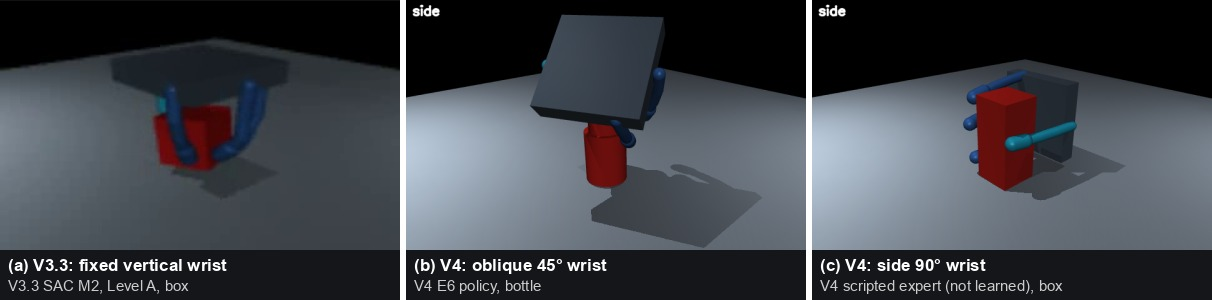
\includegraphics[width=0.80\textwidth]{fig_hand_v33_v4.jpg}\\[3pt]
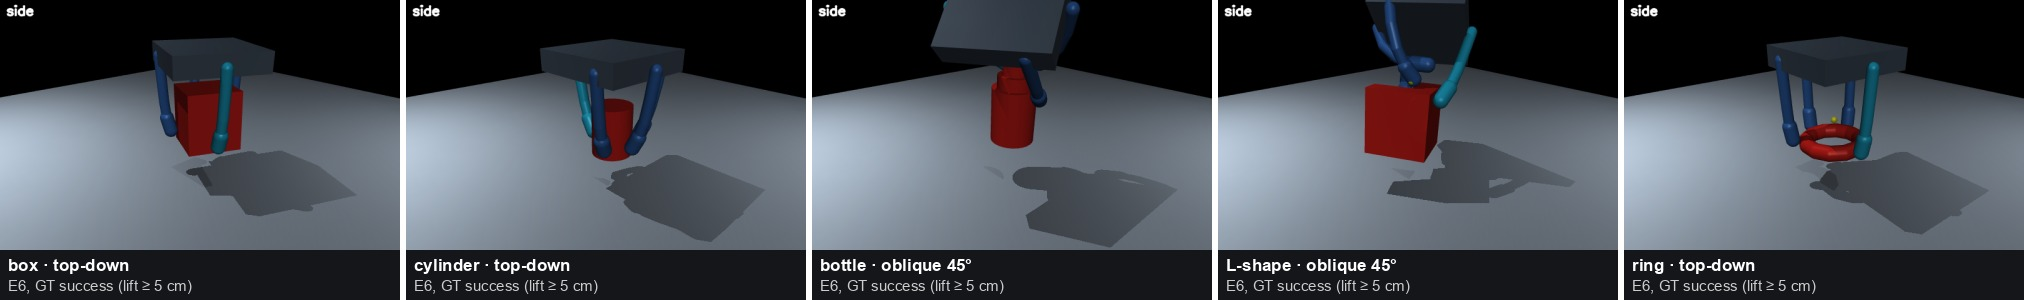
\includegraphics[width=\textwidth]{fig_objects_e6.jpg}
\caption{Real MuJoCo frames from the fixed side camera (same pose in V3.3 and V4). Top: (a) V3.3 vertical-only hand, SAC M2
policy, Level~A (\texttt{A\_train\_success.mp4}, $t=3.2$\,s); (b) V4 oblique 45$^\circ$ grasp of a bottle by the learned E6
policy (final-test seed 6715100); (c) V4 side 90$^\circ$ grasp by the \emph{scripted} expert (demo seed 7000007); no learned
policy was trained for side grasps. Bottom: the five V4 object families, each lifted by E6 on an unseen final-test episode
(frame at 5\,cm lift; seeds 6700000, 6709000, 6715100, 6721100, 6719000). Every clip was re-run and reproduced its frozen GT
outcome.}
\label{fig:hand}
\end{figure*}

\section{VisuoGrasp V4 System Architecture}\label{sec:arch}
V4 is a Python package (\path{visuograsp_v4/}): frozen dataclass configuration, MJCF scene generation with per-family
caching, a hand controller, a simulator wrapper with ground-truth bookkeeping, an analytic grasp planner, a scripted phase
machine (transit$\rightarrow$descend$\rightarrow$approach$\rightarrow$close$\rightarrow$lift$\rightarrow$hold), classical
RGB-D perception, a Gymnasium \cite{towers2024gymnasium} environment, and Stable-Baselines3 \cite{raffin2021sb3} agents.
Fig.~\ref{fig:arch} shows the run-time information flow. The actor is the only learned component at run time. Its inputs
include \priv{} information: the exact object pose/extents and ground-truth (GT) pad contacts. A camera pipeline (colour
segmentation, PCA object box, D0 contact) exists, but every policy in this report uses \texttt{obs\_mode=privileged} and
\texttt{contact\_source=gt\_oracle}; no D2 detector exists for the moving V4 wrist camera.

\begin{figure*}[t]
\centering
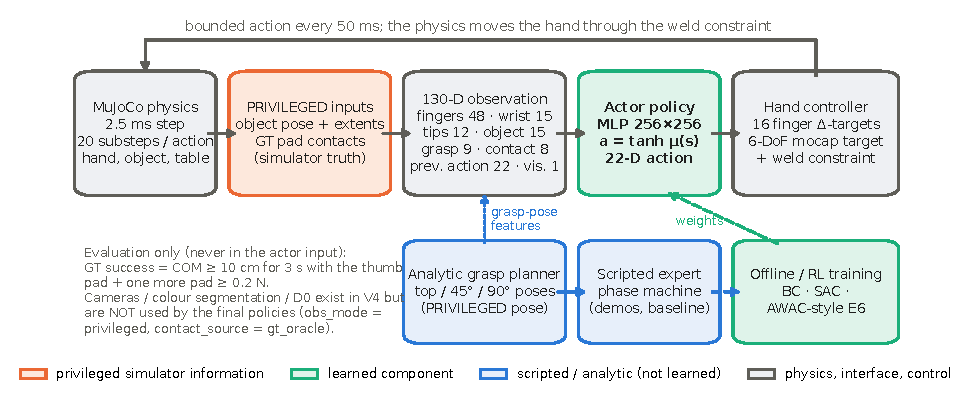
\includegraphics[width=0.92\textwidth]{fig_architecture.pdf}
\caption{V4 architecture. Orange: \priv{} simulator information in the actor input; green: learned; blue: scripted/analytic
(not learned); grey: physics and interfaces. Sources: \texttt{env.py}, \texttt{controller.py}, \texttt{grasp\_planner.py},
\texttt{scripted.py}.}
\label{fig:arch}
\end{figure*}

\section{6-DoF Robotic Control and MuJoCo Simulation}\label{sec:control}
\textbf{Hand.} The hand is a free rigid body with gravity compensation: palm $11\times11\times2.4$\,cm, four fingers with
four hinge joints each (link lengths 3.0/2.7/2.2/1.8\,cm), position servos (gains 2.5/1.8, $\pm3$\,N\,m). There are no
abduction joints. \textbf{Wrist actuation.} A massless mocap body is the commanded wrist pose; a weld equality constraint
(\texttt{solref}: 10\,ms, critical damping) pulls the hand towards it, so contacts push back and the hand carries the
object's weight without teleporting. With action $\bm a\in[-1,1]^{22}$, the targets are updated once per control step:
\begin{align}
\bm p &\leftarrow \Pi_{\mathcal W}\!\left(\bm p + 0.01\,\mathrm{m}\cdot \bm a_{16:19}\right),\label{eq:pos}\\
\bm q &\leftarrow \frac{\bm q\otimes \mathrm{Exp}(0.06\,\bm a_{19:22})}{\lVert \bm q\otimes \mathrm{Exp}(0.06\,\bm a_{19:22})\rVert},\label{eq:quat}\\
\bm\theta^{*} &\leftarrow \mathrm{clip}\!\left(\bm\theta^{*} + 0.055\,\mathrm{rad}\cdot\bm a_{0:16},\ \bm\theta_{\min},\bm\theta_{\max}\right),\label{eq:finger}
\end{align}
where $\bm p$ is the target position (world axes), $\bm q$ the target orientation quaternion (rotation in hand axes),
$\mathrm{Exp}(\bm v)=[\cos\frac{\lVert\bm v\rVert}{2},\,\sin\frac{\lVert\bm v\rVert}{2}\,\bm v/\lVert\bm v\rVert]$ the
rotation-vector-to-quaternion map, $\otimes$ quaternion multiplication \cite{shoemake1985}, and $\bm\theta^{*}$ the 16 finger servo targets.
Quaternion composition with renormalisation avoids gimbal lock and drift. Four projections follow: a workspace box
$\Pi_{\mathcal W}$, a finger-tilt limit (110$^\circ$), an anti-windup limit (target at most 2.5\,cm/0.30\,rad ahead of the
real hand) and a table-clearance check that raises the target if any palm corner or finger capsule would come within 4\,mm of
the table. The target is interpolated (lerp/slerp) over the 20 physics substeps of a control step.

\textbf{Physics.} Time step 2.5\,ms (20\,Hz control), implicit-fast integrator, elliptic friction cone, impratio 10, 65
solver and 5 no-slip iterations (as in V3.3). The finger armature was raised from $5\times10^{-5}$ to $10^{-3}$\,kg\,m$^2$
(reflected rotor inertia of a geared motor): with the old value 3 of 486 scripted diagnostic episodes ended in object
``explosions''; with the new value the same episodes ran without failure. A runaway detector (object speed $>5$\,m/s or
$|\bm x|>2$\,m) marks a \emph{numerical failure}, which always counts as a failed episode for reward and is reported separately.

\section{Object Families and Grasping Conditions}\label{sec:objects}
Five families are generated as uniform-density geometries with true centre of mass and inertia: box (cube, tall, flat),
cylinder, bottle, ring and L-shape (Fig.~\ref{fig:hand}, bottom). Each episode draws one of four scale bins (0.85--1.15), mass
0.05--0.30\,kg, sliding friction 0.5--1.2, a resting mode (upright, side, end, lying, flat) and a random yaw; the object is
placed by its support function and must pass a 0.5\,s settling check. The hand starts 26--32\,cm above the table with up to
8\,cm lateral offset and 25$^\circ$ tilt. The planner provides top-down, oblique (45$^\circ$) and side (90$^\circ$) grasp,
pre-grasp and lift poses. Side grasps need objects taller than about 8\,cm (the palm centre stays $\ge6.8$\,cm above the
table); the scripted expert reaches 30.2\% on side grasps overall and 61.3\% on the 31 feasible side episodes of its
baseline set, versus 95.1\% top-down and 60.5\% oblique (162 episodes per approach). \textbf{All learned policies were trained
and evaluated on top-down and oblique grasps only.}

\textbf{Success.} GT success (evaluation only) requires the object centre of mass to stay at least 10\,cm above its resting
height for 60 consecutive control steps (3\,s) while the thumb pad and at least one other pad press with $\ge0.2$\,N.

\section{Observation, Action, Reward and Transition Design}\label{sec:mdp}
We model grasping as a Markov decision process $\mathcal M=(\mathcal S,\mathcal A,P,r,\gamma)$ and seek
$\pi^{*}=\arg\max_\pi \mathbb E_\pi\big[\sum_{t\ge0}\gamma^{t} r_t\big]$ with $\gamma=0.99$.

\textbf{Observation} ($\mathcal S\subset\mathbb R^{130}$, normalised and clipped to $\pm10$; Table~\ref{tab:obs}). The 22-D
previous action and joint/wrist velocities form a ``history'' block that turned out to matter for imitation (Sec.~\ref{sec:results}).

\begin{table}[t]
\caption{Actor observation (130-D) and action (22-D), from \texttt{env.py}.}
\label{tab:obs}
\centering\footnotesize
\setlength{\tabcolsep}{3pt}
\begin{tabular}{@{}lr>{\raggedright\arraybackslash}p{0.57\columnwidth}@{}}
\toprule
Block & Dim & Content \\
\midrule
Fingers & 48 & joint positions, velocities, servo targets (16 each)\\
Wrist & 15 & position, 6-D rotation, linear and angular velocity\\
Fingertips & 12 & four fingertip positions (world)\\
Object (\priv) & 15 & centre, two axes, half extents, centre in hand frame\\
Grasp targets & 9 & approach command, grasp-pose position/rotation error\\
Contacts (\priv) & 8 & GT pad contacts and their temporal confirmation\\
Previous action & 22 & last executed action\\
Visibility & 1 & object-visible flag (always 1 in \priv{} mode)\\
\midrule
Action & 22 & 16 finger $\Delta$-targets, 3 translations, 3 rotations\\
\bottomrule
\end{tabular}
\end{table}

\textbf{Reward (v4r1).} Most of the reward is potential-based shaping \cite{ng1999shaping}:
\begin{multline}
r_t=\gamma\Phi(s_{t+1})-\Phi(s_t)+0.1\,\mathbb I_{\text{hold}}+10\,\mathbb I_{\text{success}}^{\text{first}}-3\,\mathbb I_{\text{drop}}^{\text{first}}\\
-0.02\min\!\Big(1,\tfrac{F_{\text{table}}}{10\,\mathrm N}\Big)-5{\cdot}10^{-4}\big(\lVert\bm a_t\rVert^2+\lVert\bm a_t-\bm a_{t-1}\rVert^2\big)-5\,\mathbb I_{\text{fail}},\label{eq:reward}
\end{multline}
\begin{multline}
\Phi=2\Big(1-\min\big(1,\tfrac{c}{0.35}\big)\Big)+\Big(1-\tfrac{\lVert\bm e_R\rVert}{\pi}\Big)+\tfrac{n_{\text{pads}}}{8}+\tfrac{\mathbb I_{\text{opp}}}{2}\\
+3\,\mathrm{clip}\Big(\tfrac{h}{0.10},0,1\Big)-\mathbb I_{h<0.02}\,\mathrm{clip}\Big(\tfrac{d_{xy}}{0.05},0,1\Big),\label{eq:phi}
\end{multline}
with corridor cost $c=\lVert\bm v\rVert+1.5\lVert\bm v_\perp\rVert\,\mathrm{clip}(1-v_\parallel/0.10,0,1)$ for the palm offset
$\bm v$ from the planned grasp pose (components along/across the approach axis), $\bm e_R$ the rotation error to the planned
orientation, $n_{\text{pads}}$ the number of contacting pads, $\mathbb I_{\text{opp}}$ thumb-plus-finger opposition, $h$ the
object lift and $d_{xy}$ the horizontal object displacement. $\Phi=0$ at terminal states. The hold bonus requires $h\ge10$\,cm
with opposition. Lift, push and table force are \priv{} simulator quantities, as in V3.3. Expressing contact and lift as
potentials removed a ``touch but never lift'' optimum of the first reward version (reward audit: that behaviour was worth a
discounted return of 1.70 versus 0.00 for doing nothing under v4r0, and $-0.12$ under v4r1).

\textbf{Transition.} One action is held for 20 substeps. Episodes terminate on a drop, the object leaving the table or a
numerical failure, and are truncated after 320 steps (16\,s); success does not terminate the episode, so that the hold is
rewarded.

\begin{figure*}[t]
\centering
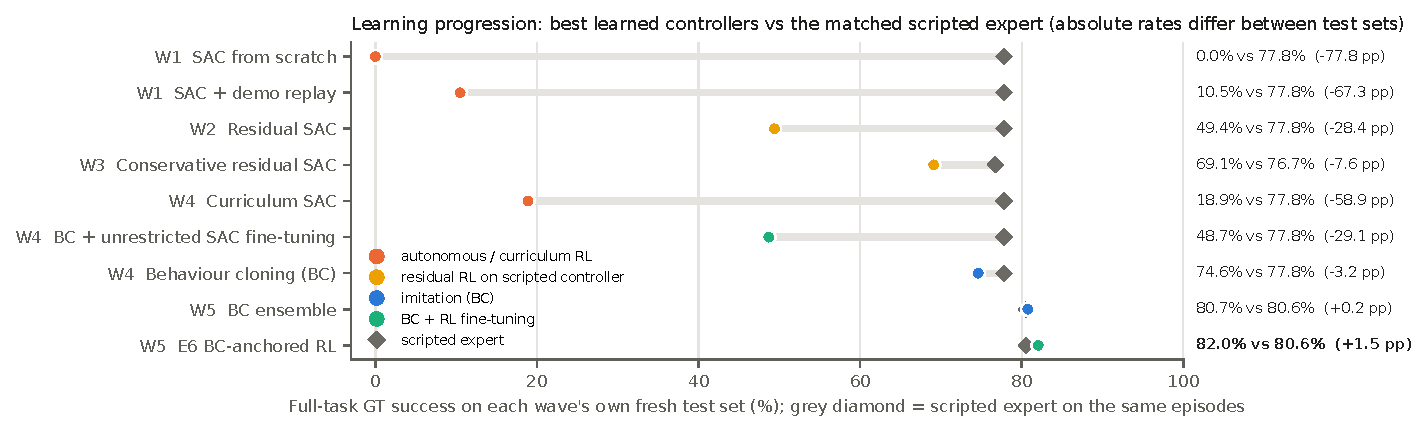
\includegraphics[width=0.95\textwidth]{fig_progression.pdf}
\caption{Best learned controllers of each wave versus the scripted expert on the same fresh test episodes (sources: wave
reports and \texttt{analysis/summary.csv}). Absolute rates differ between test sets (BC Wave~4 scored 74.6\% on 6.6M and 77.4\%
on 6.7M), so only the paired gap is comparable.}
\label{fig:prog}
\end{figure*}

\section{Reinforcement Learning and Imitation Learning Methods}\label{sec:methods}
\textbf{SAC with twin LayerNorm critics.} SAC \cite{haarnoja2018sac} trains two critics $Q_{\theta_1},Q_{\theta_2}$ (MLP
$256\times256$, LayerNorm after every hidden layer \cite{ba2016layernorm}) and a tanh-Gaussian actor
$\tilde{\bm a}=\tanh(\bm\mu_\phi(s)+\bm\sigma_\phi(s)\odot\bm\epsilon)$. Taking the minimum of two target critics limits
over-estimation \cite{fujimoto2018td3}. The one-step target and critic loss are
\begin{align}
y&=r+\gamma(1-d)\Big(\min_{j=1,2}Q_{\bar\theta_j}(s',\tilde{\bm a}')-\alpha\log\pi_\phi(\tilde{\bm a}'|s')\Big),\label{eq:target}\\
\mathcal L_Q(\theta_i)&=\mathbb E_{(s,a,r,s',d)\sim\mathcal D}\big[(Q_{\theta_i}(s,a)-y)^2\big],\quad \tilde{\bm a}'\sim\pi_\phi(\cdot|s').
\end{align}
We use $n$-step returns ($n=10$) \cite{sutton2018rl}, replacing $r$ and $\gamma$ in \eqref{eq:target} by
\begin{equation}
R^{(m)}_t=\sum_{k=0}^{m-1}\gamma^{k}r_{t+k},\qquad \gamma\rightarrow\gamma^{m},\quad m=\min(n,\ T_{\text{end}}-t),\label{eq:nstep}
\end{equation}
so that rewards propagate ten steps per update (verified in-code against direct sums, error $<2\times10^{-6}$). The actor and
the temperature $\alpha$ minimise
\begin{align}
\mathcal L_\pi(\phi)&=\mathbb E_{s,\bm\epsilon}\Big[\alpha\log\pi_\phi(\tilde{\bm a}|s)-\min_{i}Q_{\theta_i}(s,\tilde{\bm a})\Big],\\
\mathcal L(\alpha)&=\mathbb E\big[-\alpha\left(\log\pi_\phi(\tilde{\bm a}|s)+\bar{\mathcal H}\right)\big],\quad \bar{\mathcal H}=-22.
\end{align}
Hyper-parameters: learning rate $3\times10^{-4}$, batch 256, buffer $10^6$, $\tau=0.005$, one update per step.

\textbf{Residual and curriculum SAC (Waves 2--4).} Residual SAC adds bounded actor corrections to the scripted controller's
set-points (exactly the expert at zero residual, verified bit-identical). The conservative variant shrinks the bounds,
explores around zero and penalises $0.01\,\overline{r^2}$. Curriculum SAC starts episodes from scripted hand-over states
(at the grasp pose, then pre-grasp, then transit) and advances when the stage success reaches 0.5 \cite{bengio2009curriculum}.

\textbf{Behaviour cloning.} BC \cite{pomerleau1989alvinn} regresses the deterministic actor mean onto expert labels:
\begin{equation}
\mathcal L_{\text{BC}}(\phi)=\mathbb E_{(s,\bm a^{*})\sim\mathcal D_w}\Big[\tfrac{1}{22}\big\lVert\tanh\bm\mu_\phi(s)-\bm a^{*}\big\rVert^{2}\Big],\label{eq:bc}
\end{equation}
where $\mathcal D_w$ samples successful-demonstration pairs with probability proportional to $w$ (0.25 for hold/done steps,
1 otherwise, balanced between approaches). Wave~5 data: 600 clean expert episodes and 600 DART episodes \cite{laskey2017dart}
(noise $\sigma=0.05$ executed, clean label stored), 67\% oblique, 218{,}755 training pairs. BC is supervised imitation, not RL.
\textbf{Copycat fixes.} Masking the previous action (E5c/E5d), masking all history blocks (E5e/E5f) or randomly dropping
(p\,=\,0.5) and perturbing them during training (E5g/E5h, the latter with weight EMA) counter copying of the previous command
\cite{wen2020copycat,dehaan2019causal}. \textbf{BC ensemble.} The mean action of six BC actors (Wave~4 BC and the best epochs
of E5c, E5d, E5e, E5g, E5h), each with its own input masking.

\textbf{E6: BC-anchored advantage-weighted fine-tuning.} E6 starts from a BC actor and never follows $\partial Q/\partial a$.
The critics use \eqref{eq:target} with $\alpha=0$, a fixed exploration standard deviation $\sigma=0.05$, 10-step returns and
target clipping:
\begin{equation}
y=\mathrm{clip}\Big(R^{(m)}_t+\gamma^{m}(1-d)\min_j Q_{\bar\theta_j}(s_{t+m},\tilde{\bm a}'),\,-25,\,35\Big).
\end{equation}
The actor regresses towards executed actions $a$ from a mixed batch $B$ (75\% agent, 25\% demonstrations) with
advantage weights, plus a constant BC anchor on successful-demonstration pairs $D$ \cite{peng2019awr,nair2020awac,fujimoto2021td3bc}:
\begin{align}
A(s,a)&=\min_i Q_{\theta_i}(s,a)-\min_i Q_{\theta_i}\big(s,\tanh\bm\mu_\phi(s)\big),\\
w&=\frac{e^{\zeta}}{\mathrm{mean}_B\,e^{\zeta}},\quad \zeta=\min\!\Big(\frac{A}{\tau\,\sigma_B(A)},\,\ln w_{\max}\Big),\\
\mathcal L_\pi&=\frac{1}{|B|}\sum_{B}\frac{w}{22}\lVert\tanh\bm\mu_\phi(s)-a\rVert^{2}\nonumber\\
&\quad+\frac{\lambda}{|D|}\sum_{D}\frac{1}{22}\lVert\tanh\bm\mu_\phi(s_d)-a^{*}_d\rVert^{2},\label{eq:e6}
\end{align}
with $\tau=1$, $w_{\max}=20$, $\lambda=0.5$ ($A$ and $w$ detached), actor learning rate $10^{-4}$, and the actor frozen for
the first 20k updates while the critic warms up. Because the weights only re-weight actions present in the data, the policy
stays near the data support; the mean squared distance to the BC actor's actions was logged throughout.

\begin{figure*}[t]
\centering
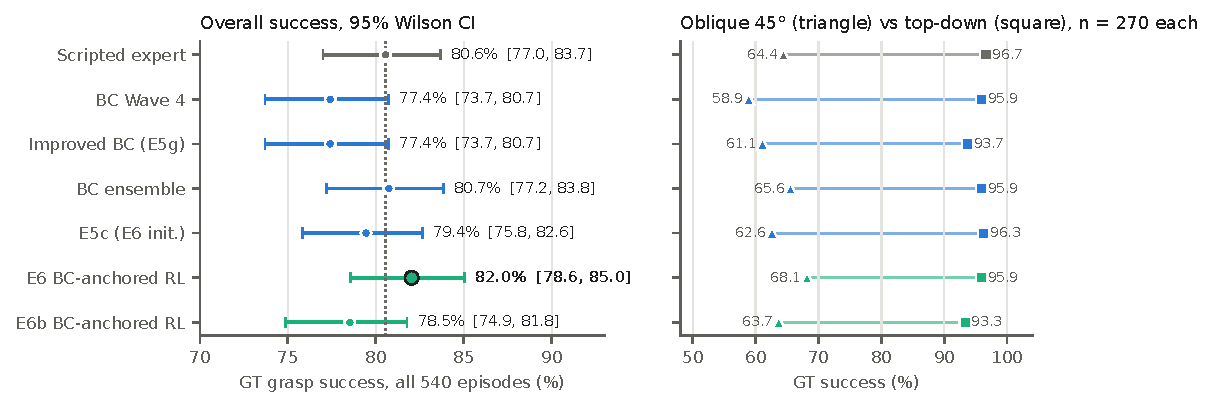
\includegraphics[width=0.95\textwidth]{fig_final_results.pdf}
\caption{Final-test GT success. Left: all 540 episodes with 95\% Wilson intervals (dotted line: scripted expert). Right:
oblique (triangles) and top-down (squares) success per controller.}
\label{fig:final}
\end{figure*}

\section{Experimental Setup}\label{sec:setup}
\textbf{Seed separation.} Demonstrations used seeds 3.4M (Wave~4) and 3.6M/3.7M (Wave~5); epoch and checkpoint selection used
DEV\_A (8.8M; 100 episodes for BC epochs, 60 per in-run RL evaluation); cross-method selection used DEV\_B (8.9M, 200
episodes); each wave used a fresh test set exactly once (5.1M, 6.1M, 6.6M; Wave~5: 6.7M). Gates, stop rules and the final
reading rule were written to JSON before the corresponding data were seen. \textbf{Final test.} 27 object cells (family
$\times$ variant $\times$ resting mode) $\times$ 2 approaches $\times$ 10 episodes = 540 episodes, identical for all seven
controllers; deterministic actions (tanh of the actor mean), PyTorch with one thread for exact reproducibility. The run was
interrupted once by an out-of-memory guard after 3{,}029 episodes and resumed; earlier records are byte-identical and the
final file contains 3{,}780 unique episodes. \textbf{Budget.} Wave~5 RL: E6 221k steps (selected checkpoint 90k, 104.8\,min),
E6b 170k steps (selected 130k, 78.1\,min), one training seed each; Wave~5 BC: eight runs, 74\,min. CPU only (Windows laptop),
Python 3.13.2, MuJoCo 3.17.0, PyTorch 2.7.1, Gymnasium 1.3.0, Stable-Baselines3 2.9.2.

\begin{figure*}[t]
\centering
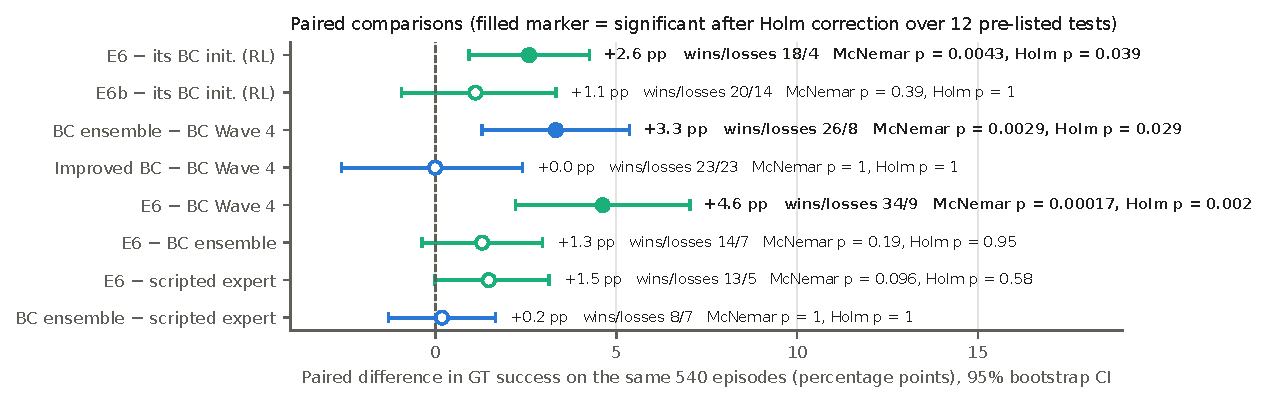
\includegraphics[width=0.95\textwidth]{fig_paired.pdf}
\caption{Paired differences with 95\% bootstrap CIs; filled markers are significant after Holm correction.}
\label{fig:paired}
\end{figure*}

\begin{figure*}[t]
\centering
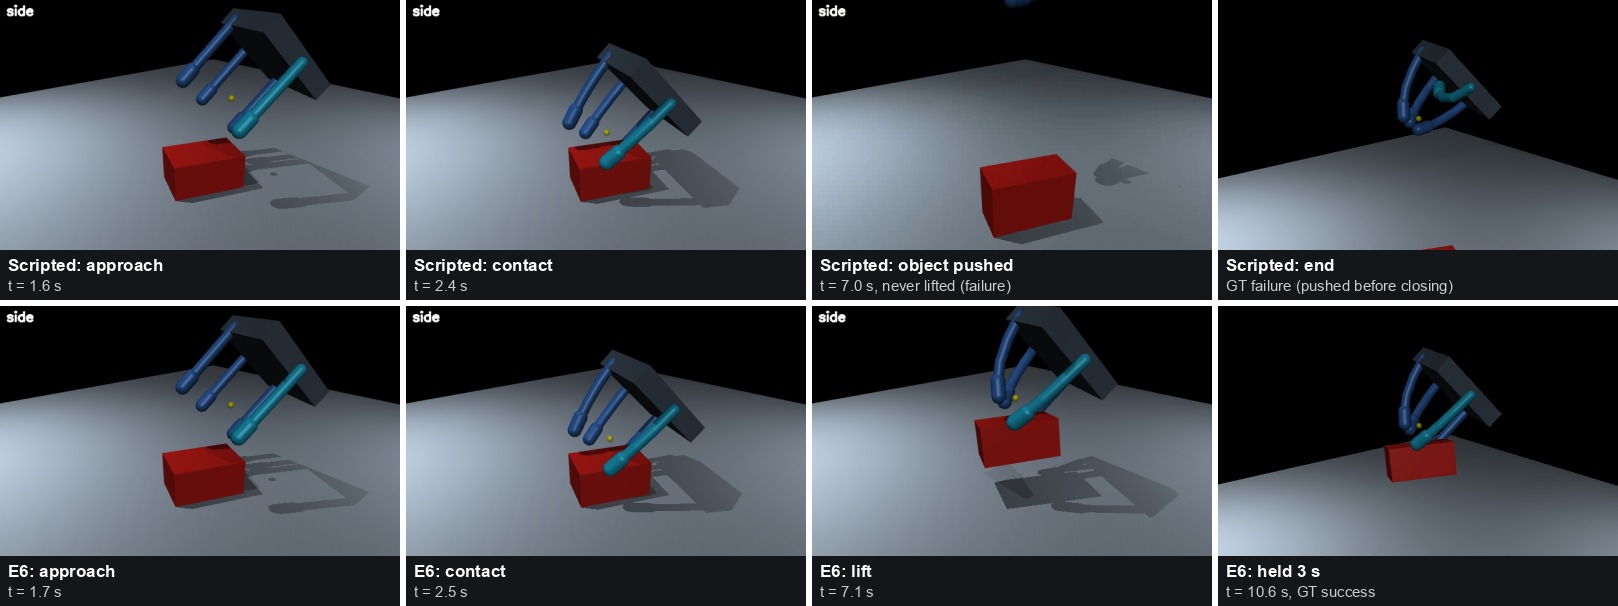
\includegraphics[width=0.97\textwidth]{fig_scripted_vs_e6.jpg}
\caption{Same unseen episode (seed 6706109, oblique, flat box) for the scripted expert (top: palm pushes the box, never
lifted) and E6 (bottom: GT success). Time stamps are simulation time.}
\label{fig:vs}
\end{figure*}

\section{Experimental Results}\label{sec:results}
\textbf{Development across waves} (Fig.~\ref{fig:prog}). Autonomous SAC reached 0\% from scratch and 10.5\% with scripted
demonstrations in its replay buffer (expert 77.8\%), mostly pushing objects away before closing. Residual SAC lowered the
expert from 77.8\% to 49.4\%; the conservative variant reduced the harm (69.1\% vs.\ 76.7\%) but never improved on the
expert. A curriculum lifted autonomous SAC to 18.9\%, a significant gain over Wave~1 but far from expert level, with 12.4\%
numerical failures. BC reached 74.6\%, while unrestricted SAC fine-tuning of BC degraded it to 48.7\%.

\textbf{Wave~5 imitation.} Plain BC on the larger data set collapsed in closed loop (DEV\_A 0.29 at epoch 10, 0.02 at epoch 30)
although the supervised error kept falling: the actor copied its previous command and lifted too slowly (59/100
\texttt{partial\_lift} for the $512^3$ network). History masking and dropout restored DEV\_A values of 0.70--0.75. The
pre-registered pick (E5g, DEV\_A 0.75) did not beat Wave~4 BC on DEV\_B (0.690 vs.\ 0.685), whereas the ensemble matched the
expert (0.730 vs.\ 0.730).

\textbf{Wave~5 RL fine-tuning.} During E6 the drift from the BC actor stayed below $3\times10^{-4}$ (mean squared action
difference), the critic stayed inside the return bound (mean Q 1.4, max $\le17$), and DEV\_A success fluctuated between 0.667
and 0.767 around the initial 0.700 (60 episodes per point). On DEV\_B the 90k checkpoint scored 0.755 vs.\ 0.730 for its
initialisation and was frozen as E6 before the final test.

\textbf{Final test} (Table~\ref{tab:final}, Fig.~\ref{fig:final}). E6 achieved the highest observed GT success, 82.0\%
[78.6, 85.0], with no numerical failures. Every controller grasps top-down objects in 93--97\% of episodes; differences arise
in oblique grasps, where E6 reaches 68.1\% versus 64.4\% for the expert and 58.9\% for Wave~4 BC. Fig.~\ref{fig:vs} shows a complete E6 grasp (bottom row: approach, contact, lift, 3-s hold) on an
episode that the expert loses by pushing the object.

\begin{table}[t]
\caption{Fresh final test (seeds 6.7M, 540 identical episodes, 270 per approach). GT success with 95\% Wilson CI.
All controllers use \priv{} simulator state. Source: \texttt{final\_test/final/analysis/summary.csv}.}
\label{tab:final}
\centering\footnotesize
\setlength{\tabcolsep}{3.2pt}
\begin{tabular}{@{}llccc@{}}
\toprule
Controller & Kind & All [95\% CI] & Top & Obl.\\
\midrule
Scripted expert & analytic & 80.6 [77.0, 83.7] & 96.7 & 64.4\\
BC Wave 4 & imitation & 77.4 [73.7, 80.7] & 95.9 & 58.9\\
Improved BC E5g & imitation & 77.4 [73.7, 80.7] & 93.7 & 61.1\\
BC ensemble & imitation & 80.7 [77.2, 83.8] & 95.9 & 65.6\\
E5c (E6 init.) & imitation & 79.4 [75.8, 82.6] & 96.3 & 62.6\\
\textbf{E6} & \textbf{BC + RL} & \textbf{82.0 [78.6, 85.0]} & 95.9 & \textbf{68.1}\\
E6b & BC + RL & 78.5 [74.9, 81.8] & 93.3 & 63.7\\
\bottomrule
\end{tabular}
\end{table}

\begin{figure*}[t]
\centering
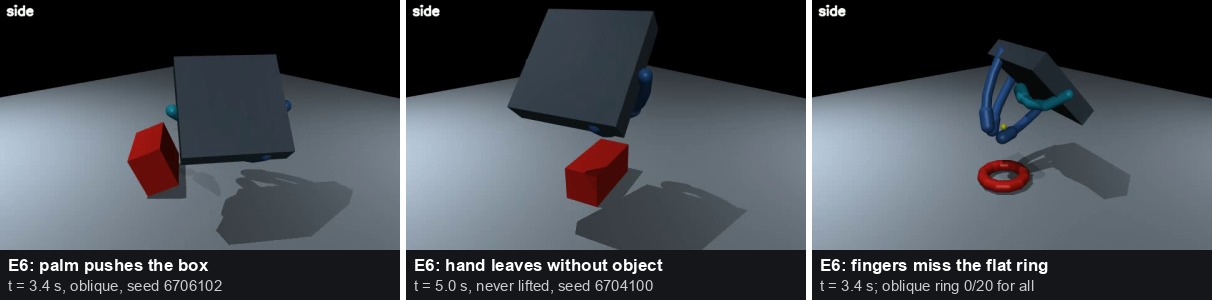
\includegraphics[width=0.86\textwidth]{fig_failures_frames.jpg}
\caption{E6 failures on unseen episodes: the palm pushes a box before closing (6706102), the hand rises without the object
(6704100), and the fingers miss a flat ring approached at 45$^\circ$ (6719100).}
\label{fig:failframes}
\end{figure*}

\section{Statistical Evaluation}\label{sec:stats}
Success rates carry Wilson intervals \cite{wilson1927}
\begin{equation}
\Big(\hat p+\tfrac{z^2}{2n}\pm z\sqrt{\hat p(1-\hat p)/n+z^2/4n^2}\Big)\Big/\big(1+z^2/n\big),\quad z=1.96.
\end{equation} Because all controllers saw
identical episodes, comparisons are paired: with $b$ episodes won only by A and $c$ only by B, the exact McNemar test
\cite{mcnemar1947} gives $p=\min\!\big(1,\,2\sum_{k=0}^{\min(b,c)}\binom{b+c}{k}2^{-(b+c)}\big)$, and a paired bootstrap
\cite{efron1993bootstrap} (10{,}000 episode resamples) gives the CI of the difference. Holm's procedure \cite{holm1979}
controls the family-wise error over the 12 overall comparisons listed before the test (Table~\ref{tab:paired},
Fig.~\ref{fig:paired}).

\begin{table}[t]
\caption{Paired comparisons on the same 540 episodes (source: \texttt{analysis/paired\_all.csv}).}
\label{tab:paired}
\centering\footnotesize
\setlength{\tabcolsep}{2.6pt}
\begin{tabular}{@{}lcccc@{}}
\toprule
A $-$ B & $\Delta$ [95\% CI] (pp) & $b/c$ & $p$ & $p_{\text{Holm}}$\\
\midrule
E6 $-$ E5c (RL) & +2.6 [+0.9, +4.3] & 18/4 & 0.0043 & \textbf{0.039}\\
E6b $-$ E5g (RL) & +1.1 [$-$0.9, +3.3] & 20/14 & 0.39 & 1.0\\
Ensemble $-$ BC W4 & +3.3 [+1.3, +5.4] & 26/8 & 0.0029 & \textbf{0.029}\\
E5g $-$ BC W4 & 0.0 [$-$2.6, +2.4] & 23/23 & 1.0 & 1.0\\
E6 $-$ BC W4 & +4.6 [+2.2, +7.0] & 34/9 & 0.00017 & \textbf{0.0020}\\
E6 $-$ ensemble & +1.3 [$-$0.4, +3.0] & 14/7 & 0.19 & 0.95\\
E6 $-$ expert & +1.5 [0.0, +3.1] & 13/5 & 0.096 & 0.58\\
Ensemble $-$ expert & +0.2 [$-$1.3, +1.7] & 8/7 & 1.0 & 1.0\\
BC W4 $-$ expert & $-$3.1 [$-$5.4, $-$0.9] & 9/26 & 0.0060 & \textbf{0.048}\\
\bottomrule
\end{tabular}
\end{table}

\textbf{Interpretation.} The RL update in E6 is significant at the 5\% level after correction ($p_{\text{Holm}}=0.039$): if
fine-tuning had no effect, a 18:4 split of the 22 discordant episodes would be unlikely. The gain concentrates on oblique
grasps (+5.6\pp, 16:1; exploratory sub-group). By contrast, 82.0\% vs.\ 80.6\% for the expert is a 13:5 split
($p=0.096$, paired CI touching 0), so superiority over the expert is \emph{not} established; neither is superiority over the
ensemble. The Wilson lower bound of E6 (78.6\%) is below 80\%, so a success rate of at least 80\% is not established either.
Four numerical failures occurred in 3{,}780 episodes, all after GT success had been reached; counting them as failures changes
no conclusion (E6 $-$ E5c +2.8\pp, $p=0.0026$).

\section{Discussion and Failure Analysis}\label{sec:discussion}
\textbf{Why autonomous and residual RL failed.} With a 22-D action and a long approach, random exploration mostly displaces the
object before any useful contact; the potential-based shaping guides the hand but the success bonus is rarely reached. Residual
SAC starts at the expert, but its early, high-entropy corrections perturb a dead-beat controller whose success depends on
precise timing, and the critic then learns from degraded states. Unrestricted SAC fine-tuning of BC followed $\partial Q/\partial a$
of a critic trained on near-expert data; even small drift increased pushing.

\textbf{Why E6 improved.} E6 never follows the critic gradient: it re-weights executed actions by their advantage and stays
anchored to expert labels. Of its 18 wins over the initialisation, 13 were episodes where the initialisation pushed the object
before closing; oblique pushes fell from 45 to 35. Fig.~\ref{fig:vs} shows the same mechanism against the expert.

\textbf{Why E6b did not reproduce it.} E6b used the same method but started from E5g (full observation with history dropout),
which is weaker top-down (93.7\%). Its changes went both ways (20 wins, 14 losses), mostly through pushing. With one training
seed per configuration we cannot separate an initialisation effect from run-to-run variance \cite{henderson2018matters}.

\textbf{Failure modes} (Fig.~\ref{fig:failfig}, Fig.~\ref{fig:failframes}). Failures are dominated by ``never lifted'' (E6: 46,
expert: 57) and ``pushed before closing'' (38 each). Oblique flat rings are never grasped by any controller (0/20): the fingers
close above the low torus. All learned policies imitate the same planner and inherit this limitation.

\begin{figure}[t]
\centering
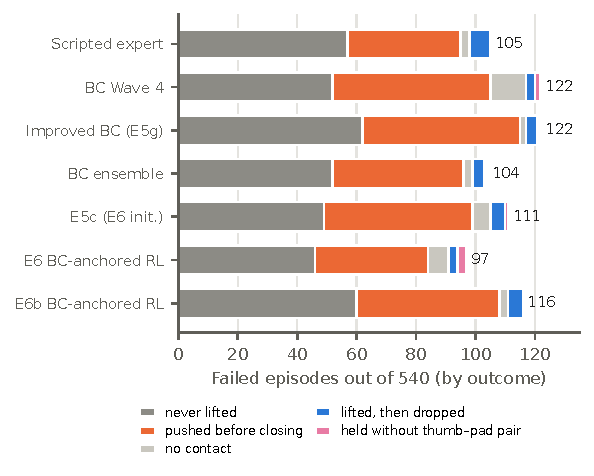
\includegraphics[width=\columnwidth]{fig_failures.pdf}
\caption{Failed episodes by outcome for each controller (source: \texttt{episodes.csv}, $\text{GT success}=0$).}
\label{fig:failfig}
\end{figure}

\section{Limitations and Future Work}\label{sec:limits}
(i) \textbf{\priv{} state, no vision.} Object pose and pad contacts come from the simulator; the course's central requirement,
vision-confirmed contact inside the RL loop, is met by V3.3 but not by V4. Porting the D2 detector to the moving wrist camera
and training with \texttt{obs\_mode=vision} is the main next step. (ii) \textbf{One training seed} per RL configuration, and the
E6 gain was not replicated; 3--5 seeds are needed. (iii) \textbf{No significant gain over the expert}, and the learned policies
depend on an analytic planner. (iv) \textbf{Coverage:} side grasps are scripted only, oblique rings fail, and no YCB or
real-robot evaluation was done. (v) \textbf{Simulation only}, with one set of physics parameters.

\section{Conclusion}\label{sec:conclusion}
VisuoGrasp V4 turns a vertical-only grasping setup into physically controlled 6-DoF grasping with a 22-D action space and five
object families. Across five waves, RL from reward alone, as residual corrections, or with a curriculum did not reach the
\priv{} scripted expert. Imitation combined with a conservative, expert-anchored RL update did: E6 reached 82.0\% GT success
on 540 unseen episodes and significantly improved its BC initialisation ($p_{\text{Holm}}=0.039$), while remaining
statistically equivalent to the expert. Making the policy vision-based and replicating the RL gain across seeds are the
essential next steps.

\FloatBarrier
\bibliographystyle{IEEEtran}
\bibliography{references}

\appendix
\sloppy
\subsection{Reproducibility}
Frozen inputs: \path{rl/wave5/frozen_policies/manifest.json} (SHA-256 of E6, E6b and all BC actors) and
\path{rl/wave5/RESULTS_FROZEN_SHA256.txt} (78 result files). Per-episode CSVs, analysis scripts and the pre-registered
rules (\path{wave5_plan_and_rules.json}, \path{final_test/final_decision_rule.json}) are in
\path{visuograsp_v4/outputs/rl/wave5/}. Every figure of a simulated episode was re-run with the frozen policy and its GT
outcome matched the frozen record (\path{final_defense/media/rerendered/rerender_manifest.csv}). The final test was
interrupted once by memory protection and resumed with \path{--resume}; integrity checks are in
\path{final_test/final/resume_log.txt}.

\subsection{E6 hyper-parameters}
Initial actor: E5c epoch 10 (previous action masked); critics: LayerNorm MLP $256\times256$, lr $3\times10^{-4}$, $n=10$,
$\gamma=0.99$, $\tau_{\text{polyak}}=0.005$, batch 256 (25\% demonstrations from 367{,}673 transitions), target clip $[-25,35]$;
actor: lr $10^{-4}$, frozen for 20k updates, $\sigma=0.05$ fixed, $\alpha=0$, $\tau=1$, $w_{\max}=20$, $\lambda=0.5$;
evaluation every 10k steps on 60 DEV\_A episodes; stop rule: two consecutive evaluations below the BC reference $-8$\pp; gates at
50k ($\ge$ reference) and 150k ($>$ reference + 3\pp).

\end{document}
